\documentclass[10pt,a4paper,conference]{IEEEtran}
\usepackage{amsmath,amssymb}
\usepackage{graphicx}
\usepackage{algorithm}
\usepackage{algorithmic}
\usepackage{url}
\usepackage{caption}
\usepackage{subcaption}
\usepackage{booktabs}
\usepackage{enumitem}

% Figures are stored under experiment/*/results/. Compile from the repository root
% (e.g. \texttt{latexmk -pdf main\_full.tex}) so these relative paths resolve.
\graphicspath{{experiment/A/results/}{experiment/B/results/}{experiment/C/results/}{experiment/D/results/}}

\title{Importance Sampling for Artificial Intelligence}
\author{
    \IEEEauthorblockN{Mathematics for AI Course Project}
    \IEEEauthorblockA{Yuncong Wang, Xiangqian Wang, Qingfeng Li}
    }

\begin{document}
\maketitle

\begin{abstract}
Importance Sampling (IS) is a fundamental Monte Carlo technique for estimating expectations under intractable target distributions. Instead of sampling directly from the target distribution \(p(x)\), which is often difficult or impossible, IS samples from an easy-to-sample proposal distribution \(q(x)\) and corrects the bias using importance weights. This report introduces the mathematical derivation, core properties, applications in reinforcement learning, and four reproducible experiments aligned with our code. We show that a proposal matched to \(|f|p\) can collapse variance on a benchmark integral; that self-normalized IS compares fairly to direct Monte Carlo and rejection sampling on a Gaussian mixture; that a heavy-tailed Student-\(t\) proposal stabilizes weights for a tail-sensitive functional where a narrow Gaussian proposal does not; and that in high dimensions even a small proposal mean shift drives the effective sample size (ESS) toward zero while sampling from the target itself leaves ESS intact. Importance Sampling remains essential for off-policy evaluation, Bayesian inference, and rare-event simulation in modern AI.
\end{abstract}

\section{INTRODUCTION}
In machine learning and statistical computing, we often aim to compute the expectation of a function \(f(x)\) under a target distribution \(p(x)\):
\[
\mathbb{E}_{p}[f(x)] = \int f(x)\,p(x)\,dx.
\]
Direct sampling from \(p(x)\) is frequently infeasible due to complex structures, high dimensionality, or lack of a generative procedure. Importance Sampling resolves this by reusing samples from a proposal \(q(x)\) that is easy to sample, then reweighting them to recover the target expectation.

\section{MATHEMATICAL FOUNDATION}
\subsection{Core Derivation}
The key step is to rewrite the expectation by multiplying and dividing by \(q(x)\):
\begin{equation}
\begin{aligned}
\mathbb{E}_{p}[f(x)] 
&= \int f(x)\,p(x)\,dx \\
&= \int f(x)\,\frac{p(x)}{q(x)}\,q(x)\,dx \\
&= \mathbb{E}_{q}\!\left[\,f(x)\cdot \frac{p(x)}{q(x)}\,\right].
\end{aligned}
\end{equation}

\subsection{Importance Weight}
We define the \emph{importance weight}:
\[
w(x) = \frac{p(x)}{q(x)}.
\]

\subsection{Monte Carlo Estimation}
Given \(N\) independent samples \(x_i \sim q(x)\), the IS estimator is:
\begin{equation}
\hat{\mathbb{E}}_{p}[f] = \frac{1}{N}\sum_{i=1}^{N} f(x_i)\,w(x_i).
\end{equation}
This estimator is unbiased if \(q(x) > 0\) whenever \(p(x) > 0\).

\subsection{Normalized Importance Sampling and ESS}
When only an unnormalized \(\tilde{p}(x)=Z\,p(x)\) is available, self-normalized (normalized) IS uses \(\tilde{w}_i=\tilde{p}(x_i)/q(x_i)\) and
\begin{equation}
\hat{\mu}_{\mathrm{NIS}}=\frac{\displaystyle\sum_{i=1}^{N} f(x_i)\,\tilde{w}_i}{\displaystyle\sum_{i=1}^{N} \tilde{w}_i}.
\end{equation}
To diagnose weight degeneracy we report the \emph{effective sample size} in the usual form \(\mathrm{ESS}=(\sum_i w_i)^2/\sum_i w_i^2\) (for unnormalized weights the same formula applied to \(\tilde{w}_i\) is common practice) and the ratio \(\mathrm{ESS}/N\).

\section{APPLICATION: OFF-POLICY REINFORCEMENT LEARNING}
Importance Sampling is the foundation of modern off-policy RL algorithms such as PPO and TRPO. It allows evaluating a new policy \(\pi_{\text{new}}\) using trajectories collected from an old policy \(\pi_{\text{old}}\):
\begin{equation}
\begin{aligned}
J(\pi_{\text{new}}) &= \mathbb{E}_{\tau\sim\pi_{\text{old}}}\Bigl[\,R(\tau) \\
&\qquad {}\cdot \frac{p_{\text{new}}(\tau)}{p_{\text{old}}(\tau)}\,\Bigr],
\end{aligned}
\end{equation}
where \(\tau\) is a trajectory, \(R(\tau)\) is the reward, and the weight corrects the distribution shift between policies.

\section{EXPERIMENTS AND RESULTS}
All experiments use \texttt{Python}~3 with \texttt{NumPy}/\texttt{SciPy}, random seed \(42\), and the scripts under \texttt{experiment/A/src/}, \ldots, \texttt{experiment/D/src/}. Sample sizes and repetition counts \(M\) match those scripts unless noted.

\subsection{Experiment A: Variance under optimal, uniform, and mismatched proposals}
\textbf{Problem.} We estimate \(I=\int_0^1 e^x\,dx=e-1\) as \(\mathbb{E}_p[f(X)]\) with \(p(x)=\mathbb{I}_{[0,1]}(x)\) and \(f(x)=e^x\). We compare: (i)~direct Monte Carlo with \(X\sim\mathrm{Unif}(0,1)\); (ii)~IS with \(q_{\mathrm{opt}}(x)=(e-1)^{-1}e^x\) on \([0,1]\), so \(f(x)w(x)\) is constant and the theoretical variance is zero up to floating-point error; (iii)~IS with \(q_{\mathrm{bad}}(x)=2x\) on \([0,1]\), which places little mass near \(0\) where \(p/q\) is large.

\textbf{Procedure.} Sample sizes \(N\in\{10,30,100,300,1000,3000,10000\}\). For each~\(N\), we run \(M=1000\) independent replications and record the empirical variance of the estimate across replications and the mean estimate versus~\(N\).

\textbf{Results.} Figure~\ref{fig:expA} shows variance on log--log axes and mean convergence. Optimal IS tracks the true value \(e-1\) with negligible spread even for small \(N\). Direct MC follows the usual \(\propto 1/N\) variance decay. The bad linear proposal yields higher variance than direct MC because weights explode when samples fall near \(0\). Figure~\ref{fig:expAweights} contrasts weight histograms for one run at \(N{=}1000\): optimal weights concentrate tightly, whereas the bad proposal induces a long right tail in \(w(x)=1/(2x)\) (plot clipped for readability).

\begin{figure}[!t]
\centering
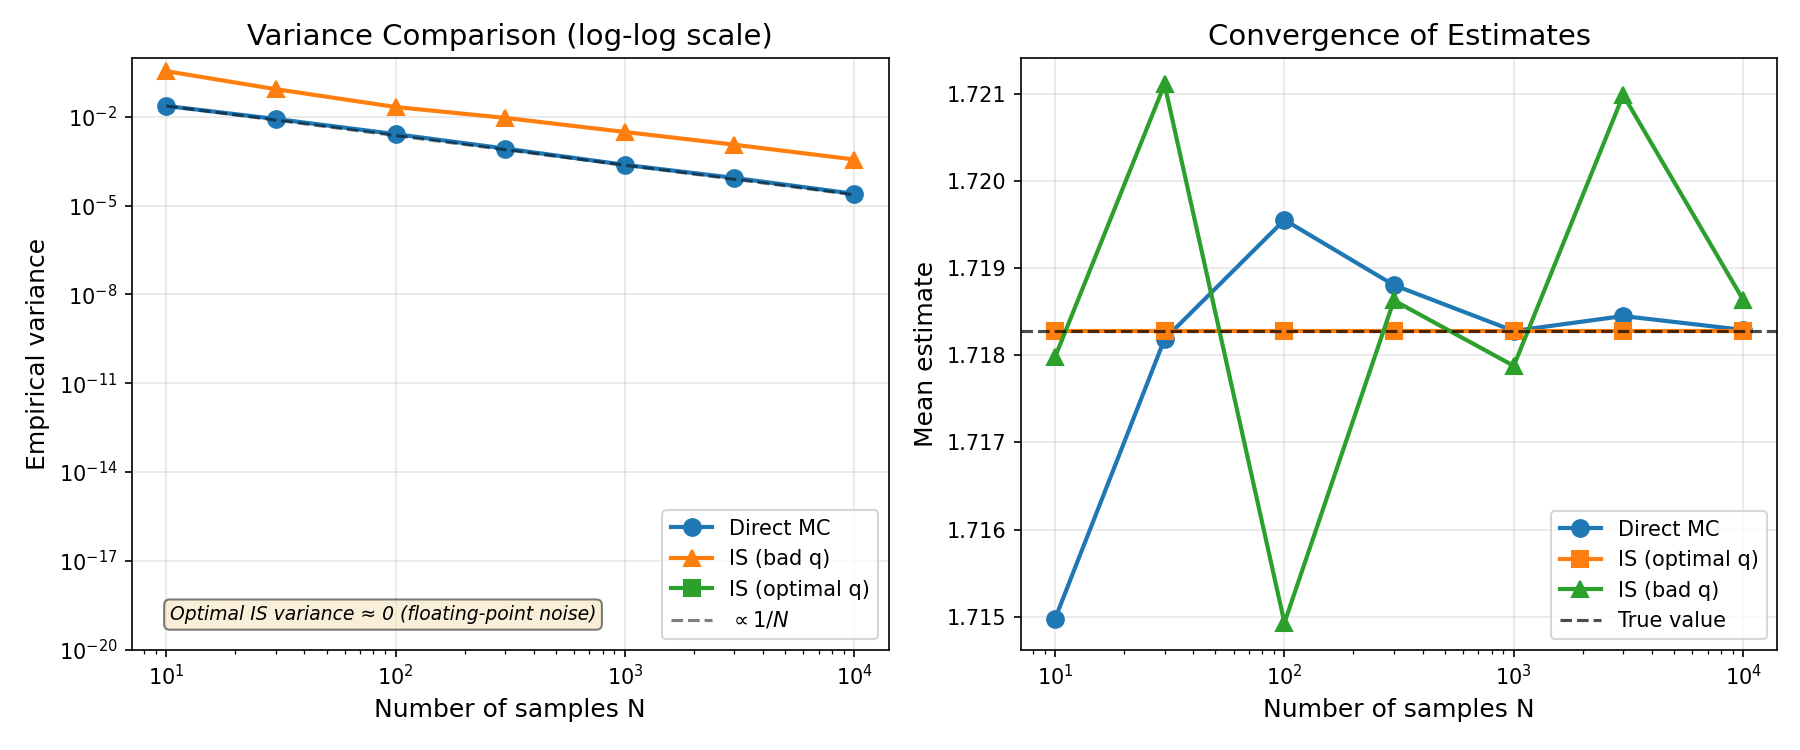
\includegraphics[width=\columnwidth]{experiment1_results.png}
\caption{Experiment~A: empirical variance vs.\ \(N\) (left) and mean estimate vs.\ \(N\) (right) for direct MC, optimal IS, and mismatched IS.}
\label{fig:expA}
\end{figure}

\begin{figure}[!t]
\centering
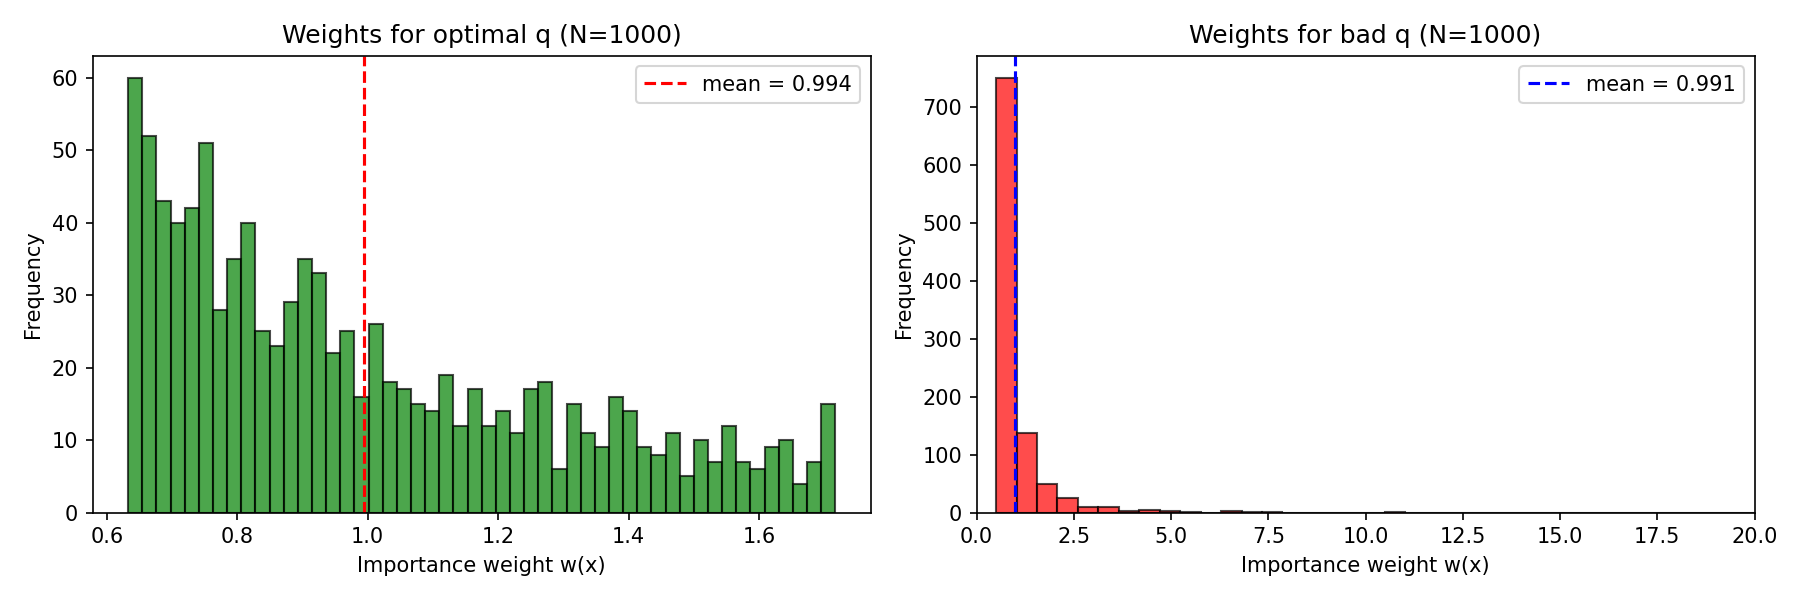
\includegraphics[width=\columnwidth]{experiment1_weights.png}
\caption{Experiment~A: distributions of importance weights for optimal vs.\ bad proposals (\(N{=}1000\), single run).}
\label{fig:expAweights}
\end{figure}

\subsection{Experiment B: Gaussian mixture---direct sampling, rejection sampling, and NIS}
\textbf{Target.} \(p(x)=0.3\,\mathcal{N}(x;4,1)+0.7\,\mathcal{N}(x;7,0.5)\), where the second Gaussian has variance \(0.5\) (\texttt{scipy} scale \(\sqrt{0.5}\)). The exact mean is \(\mathbb{E}_p[X]=0.3\cdot 4+0.7\cdot 7=6.1\).

\textbf{Methods.} (i)~Direct Monte Carlo: sample from the mixture. (ii)~Rejection sampling: proposal \(\mathcal{N}(6,3^2)\) with envelope constant \(M=2.5\) (verified to dominate \(p/q_{\mathrm{rs}}\)). We record the fraction of proposals accepted when generating \(N\) samples. (iii)~Self-normalized IS: proposal Student-\(t\) with \(\nu=5\), location \(6\), scale \(2\); estimate \(\sum_i X_i w_i/\sum_i w_i\) with \(w_i=p(x_i)/q(x_i)\).

\textbf{Procedure.} Sample sizes \(N\in\{100,300,1000,3000,10000\}\); \(M=500\) replications per~\(N\).

\textbf{Results.} Figure~\ref{fig:expBhist} compares normalized histograms to \(p(x)\): direct sampling matches the bimodal shape; rejection sampling matches after accepting a random subset; IS matches the target density when bins are weighted by \(w_i\). Figure~\ref{fig:expBvar} shows empirical variance of the mean estimate versus \(N\): all three methods improve with \(N\), but rejection sampling incurs extra proposals when acceptance is below one. Figure~\ref{fig:expBmean} confirms unbiased mean convergence toward \(6.1\) for all three estimators.

\begin{figure}[!t]
\centering
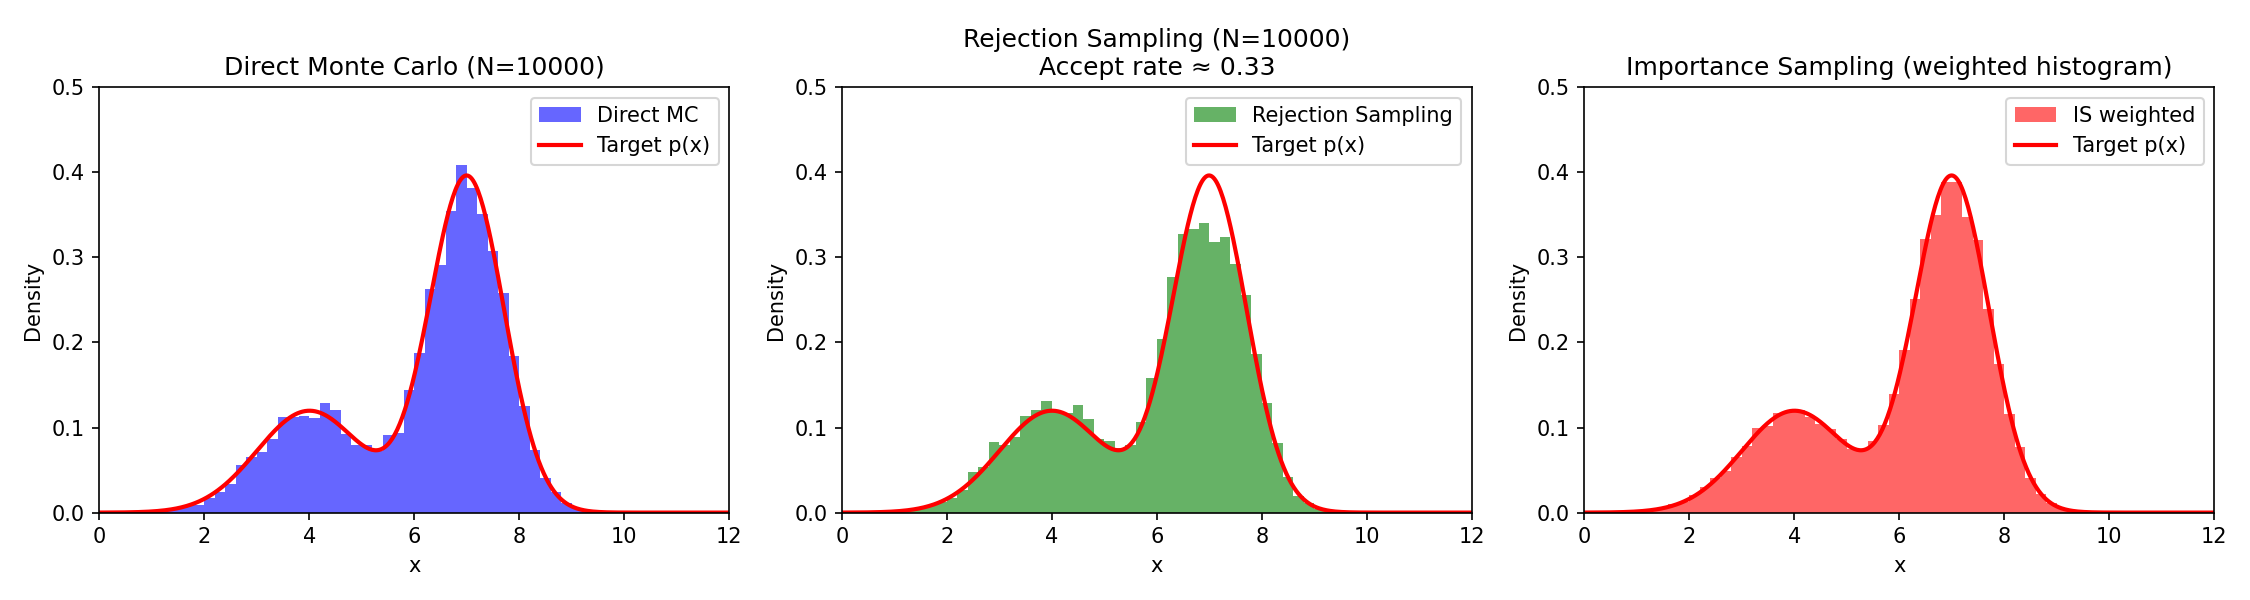
\includegraphics[width=\columnwidth]{experiment2_histograms.png}
\caption{Experiment~B: density recovery---direct samples, rejection samples, and weighted IS histograms vs.\ \(p(x)\).}
\label{fig:expBhist}
\end{figure}

\begin{figure}[!t]
\centering
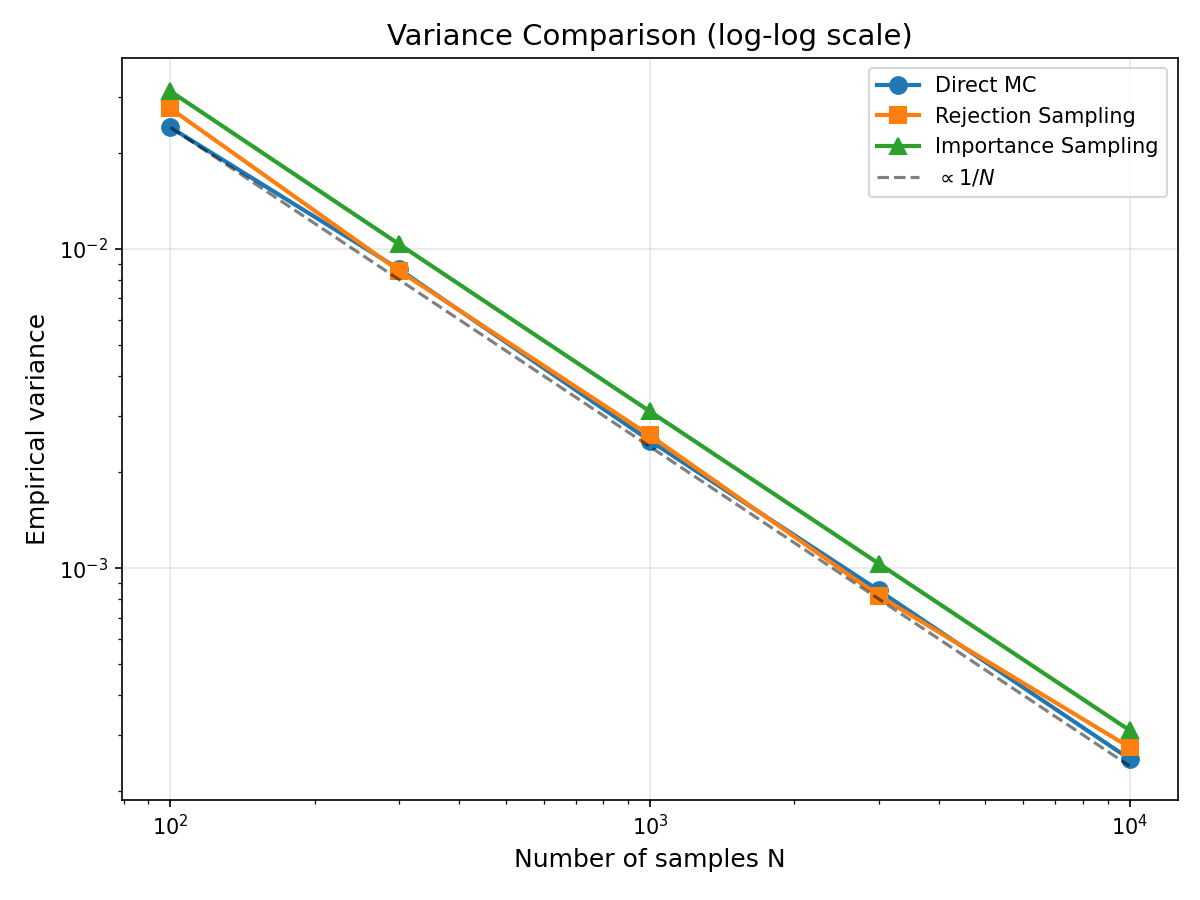
\includegraphics[width=\columnwidth]{experiment2_variance.png}
\caption{Experiment~B: empirical variance of the estimated mean vs.\ sample size \(N\) (log--log).}
\label{fig:expBvar}
\end{figure}

\begin{figure}[!t]
\centering
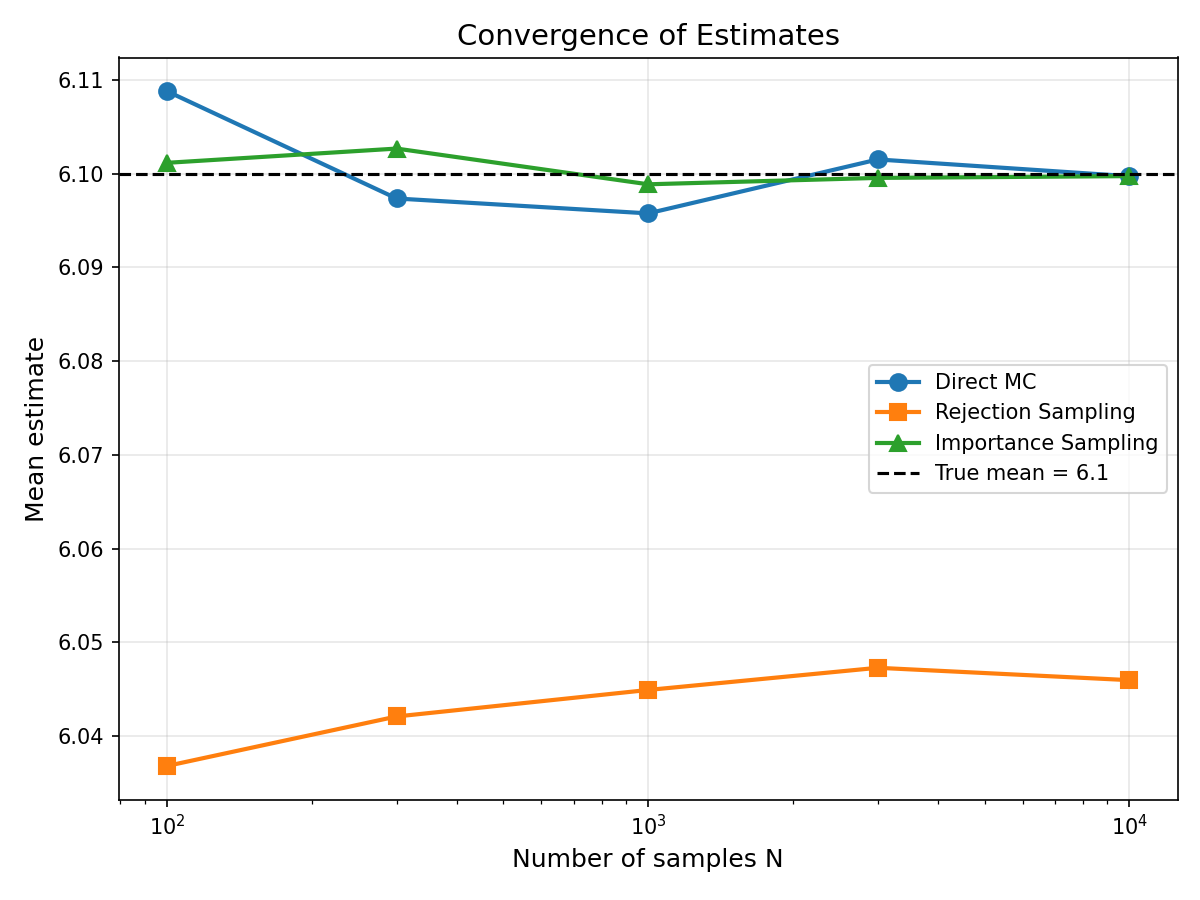
\includegraphics[width=\columnwidth]{experiment2_means.png}
\caption{Experiment~B: mean estimate vs.\ \(N\) compared to the true mean \(6.1\).}
\label{fig:expBmean}
\end{figure}

\subsection{Experiment C: Tail-sensitive functional under a mixture target}
\textbf{Target and quantity.} We use
\begin{equation}
\begin{aligned}
p(x) &= 0.9\,\mathcal{N}(x;0,1) \\
&{}+ 0.1\,\mathcal{N}(x;10,0.5^2).
\end{aligned}
\end{equation}
and estimate \(\theta=\mathbb{E}_p\bigl[X\,\mathbb{I}\{X>8\}\bigr]\). The reference value \(\theta\approx 0.999975\) is obtained by numerical integration (\texttt{scipy.integrate.quad}).

\textbf{Proposals.} Good: Student-\(t\) with \(\nu=3\), location \(8\), scale \(1.5\) (heavier tails). Bad: \(\mathcal{N}(8,1)\). We use the standard unbiased IS estimator \(\hat\theta=\frac{1}{N}\sum_i X_i\mathbb{I}\{X_i>8\}\,w_i\) with \(w_i=p(x_i)/q(x_i)\).

\textbf{Procedure.} Sample sizes \(N\in\{2000,5000,\ldots,200000\}\) as in the script; \(M=200\) replications per~\(N\).

\textbf{Results.} Figure~\ref{fig:expCvar} shows variance across replications: the heavy-tailed proposal yields variance that shrinks steadily with \(N\), whereas the Gaussian proposal produces much larger and noisier variance. Figure~\ref{fig:expCmean} shows mean estimates versus \(N\): the good proposal tracks \(\theta\) closely, while the bad proposal oscillates. Figure~\ref{fig:expCw} displays histograms of weights restricted to samples with \(X>8\); the bad proposal induces a heavier tail of extreme weights. Figure~\ref{fig:expCdens} compares \(p(x)\) to proposal densities on a log scale for tail context.

\begin{figure}[!t]
\centering
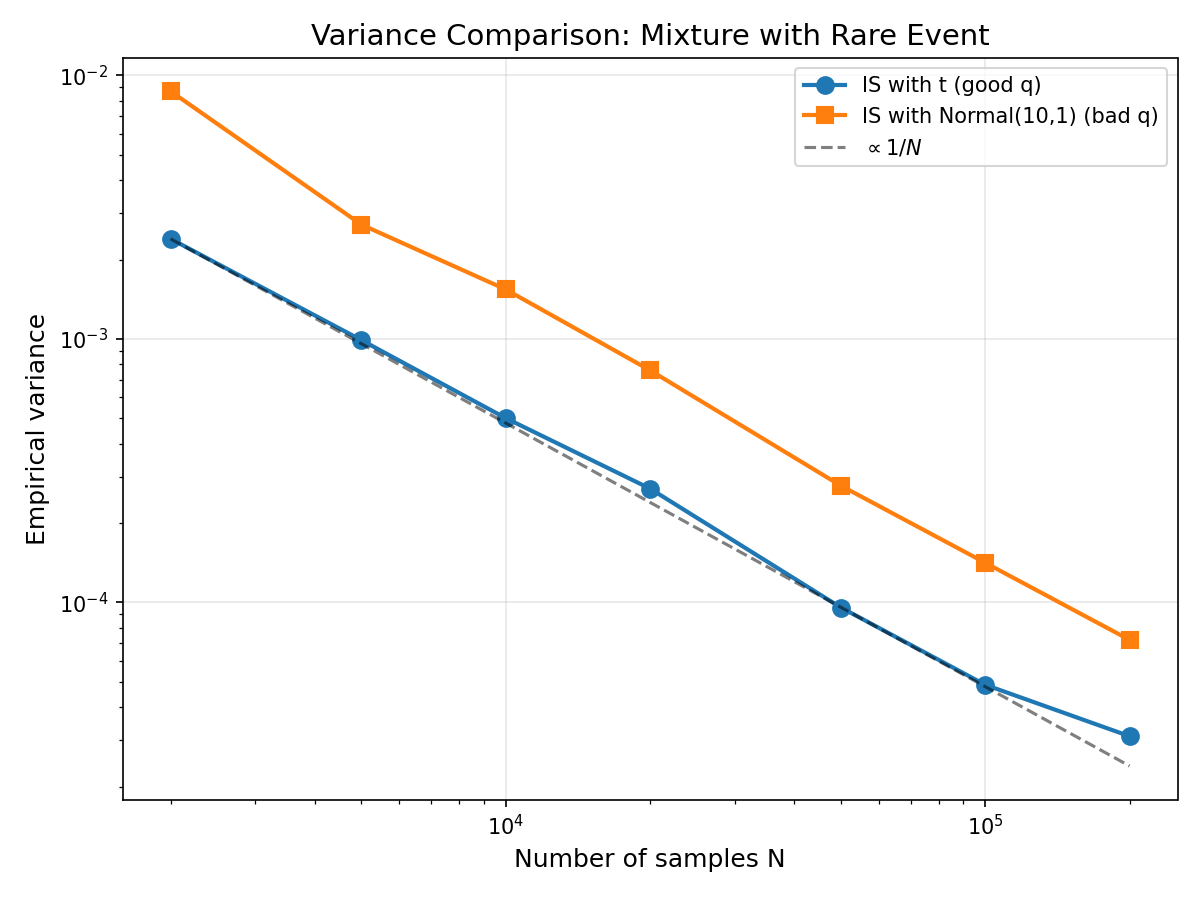
\includegraphics[width=\columnwidth]{tail_exp_variance.png}
\caption{Experiment~C: empirical variance of \(\hat\theta\) vs.\ \(N\) for heavy-tailed vs.\ Gaussian proposals.}
\label{fig:expCvar}
\end{figure}

\begin{figure}[!t]
\centering
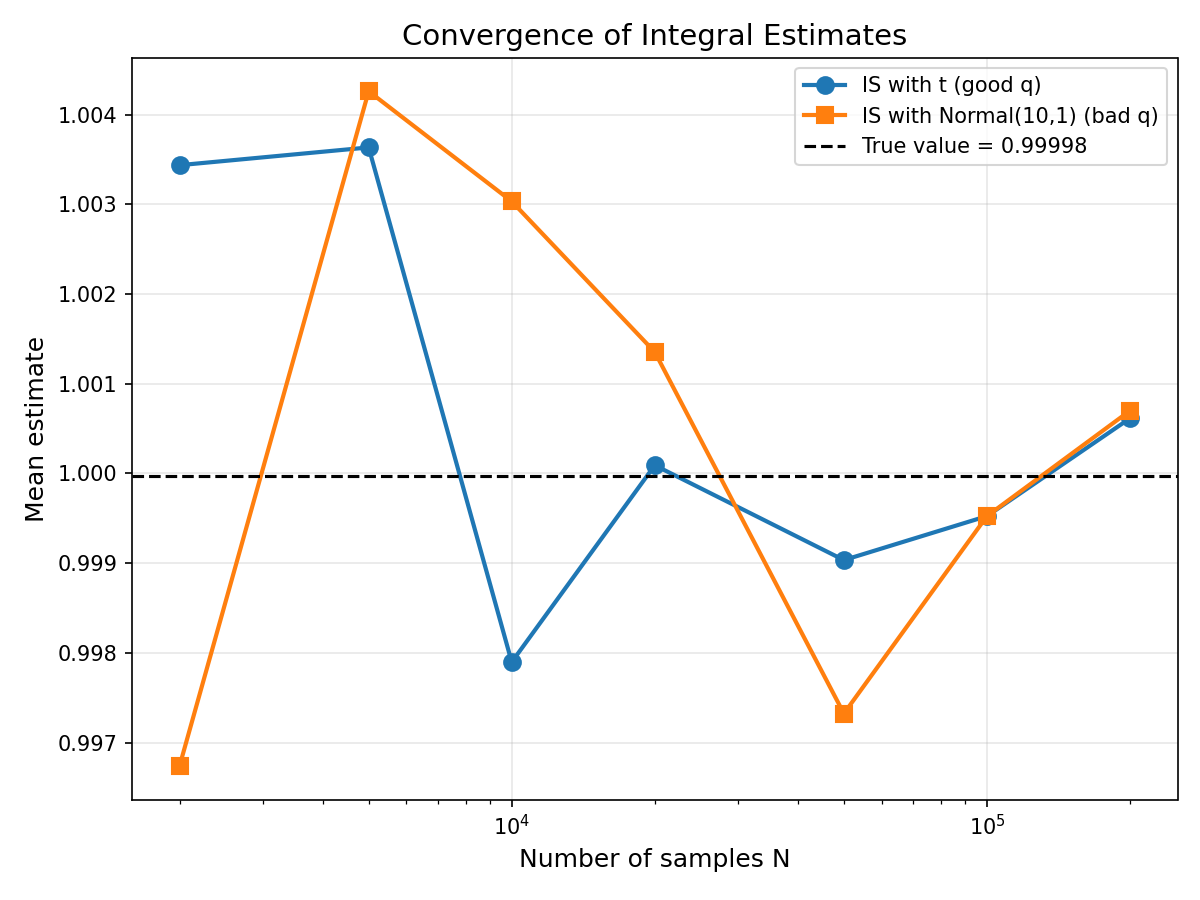
\includegraphics[width=\columnwidth]{tail_exp_means.png}
\caption{Experiment~C: mean estimate of \(\theta\) vs.\ \(N\) vs.\ numerical ground truth.}
\label{fig:expCmean}
\end{figure}

\begin{figure}[!t]
\centering
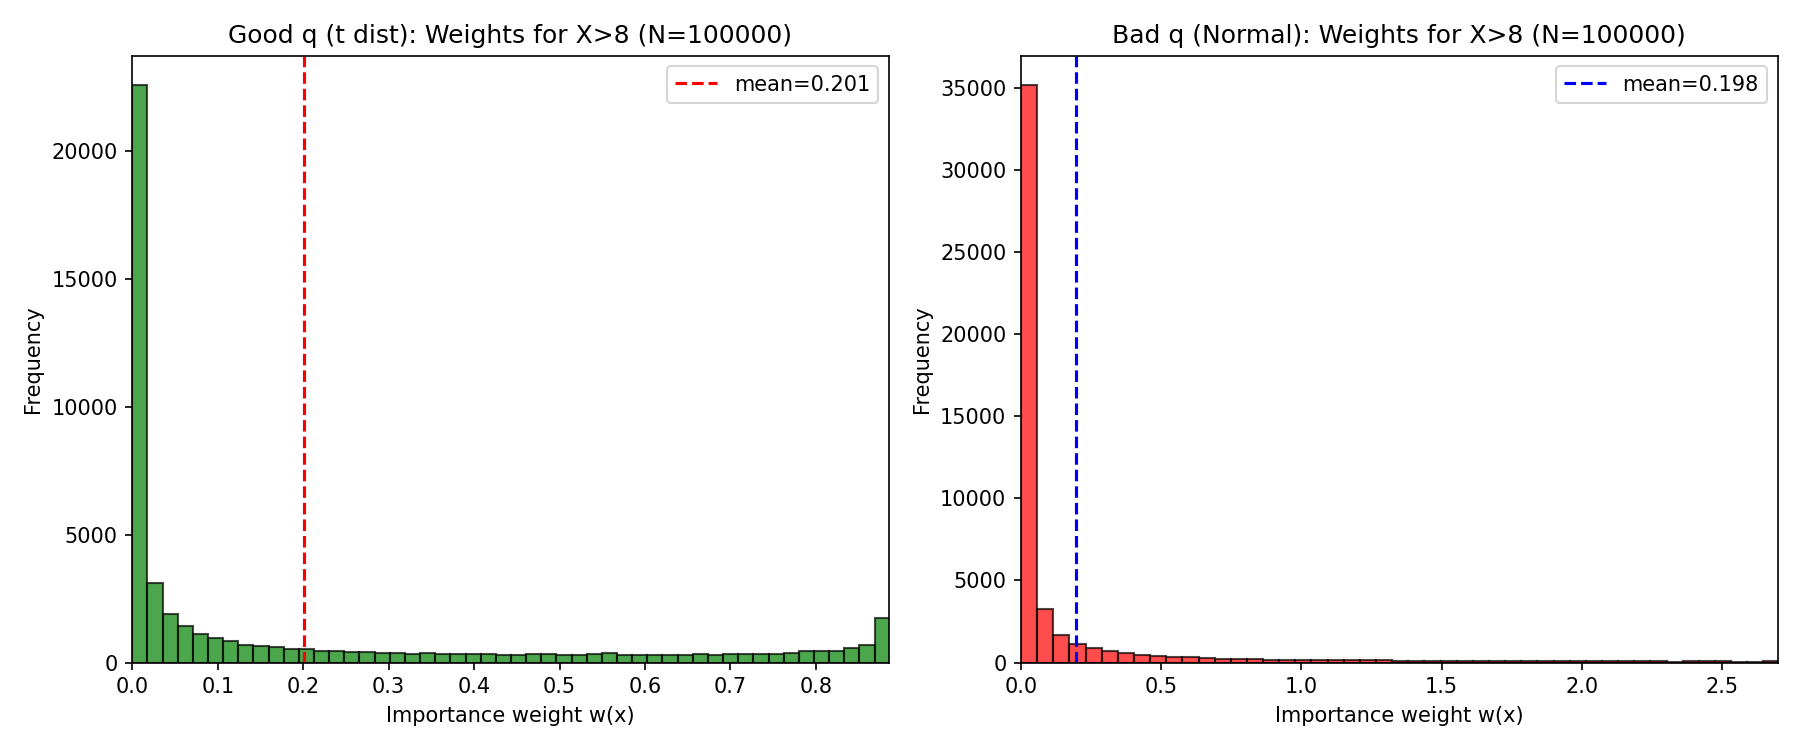
\includegraphics[width=\columnwidth]{tail_exp_weights.png}
\caption{Experiment~C: weight histograms for samples with \(X>8\) (single large-\(N\) run; axes clipped for display).}
\label{fig:expCw}
\end{figure}

\begin{figure}[!t]
\centering
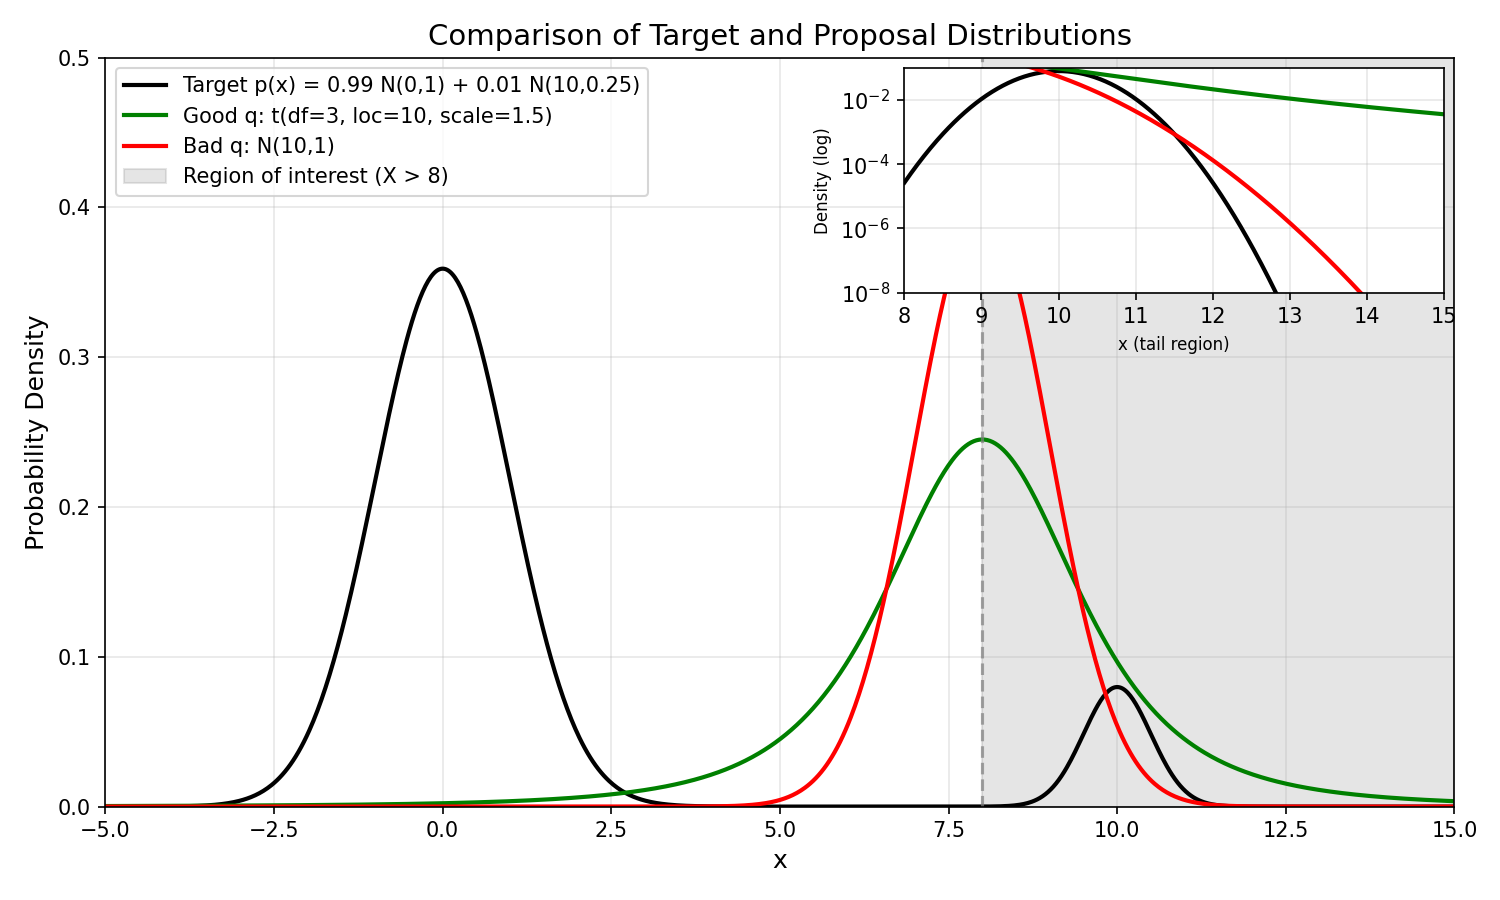
\includegraphics[width=\columnwidth]{tail_exp_density_comparison.png}
\caption{Experiment~C: target mixture \(p(x)\) vs.\ proposal densities (log scale).}
\label{fig:expCdens}
\end{figure}

\subsection{Experiment D: High-dimensional ESS---ideal vs.\ offset Gaussian proposal}
\textbf{Setup.} Target \(p=\mathcal{N}(\mathbf{0},\mathbf{I}_d)\). We draw \(m=2000\) samples from two proposals: (i)~\(q=p\) (ideal), giving weights identically one up to numerical error; (ii)~\(q=\mathcal{N}(a\mathbf{1},\mathbf{I}_d)\) with \(a=0.5\) on every coordinate, inducing a systematic mismatch that grows with \(d\).

\textbf{Metric.} We report \(\mathrm{ESS}/m\) with \(\mathrm{ESS}=(\sum_i w_i)^2/\sum_i w_i^2\) and \(w_i=p(x_i)/q(x_i)\).

\textbf{Results.} Figure~\ref{fig:expD} shows \(\mathrm{ESS}/m\) vs.\ \(d\in\{1,2,5,10,50,100,1000\}\) on a log scale. Under \(q=p\), the ratio stays near one for all tested dimensions. Under the offset proposal, \(\mathrm{ESS}/m\) collapses orders of magnitude as \(d\) increases, illustrating weight concentration and the difficulty of naive IS in high dimensions even when \(p\) and \(q\) are both simple Gaussians.

\begin{figure}[!t]
\centering
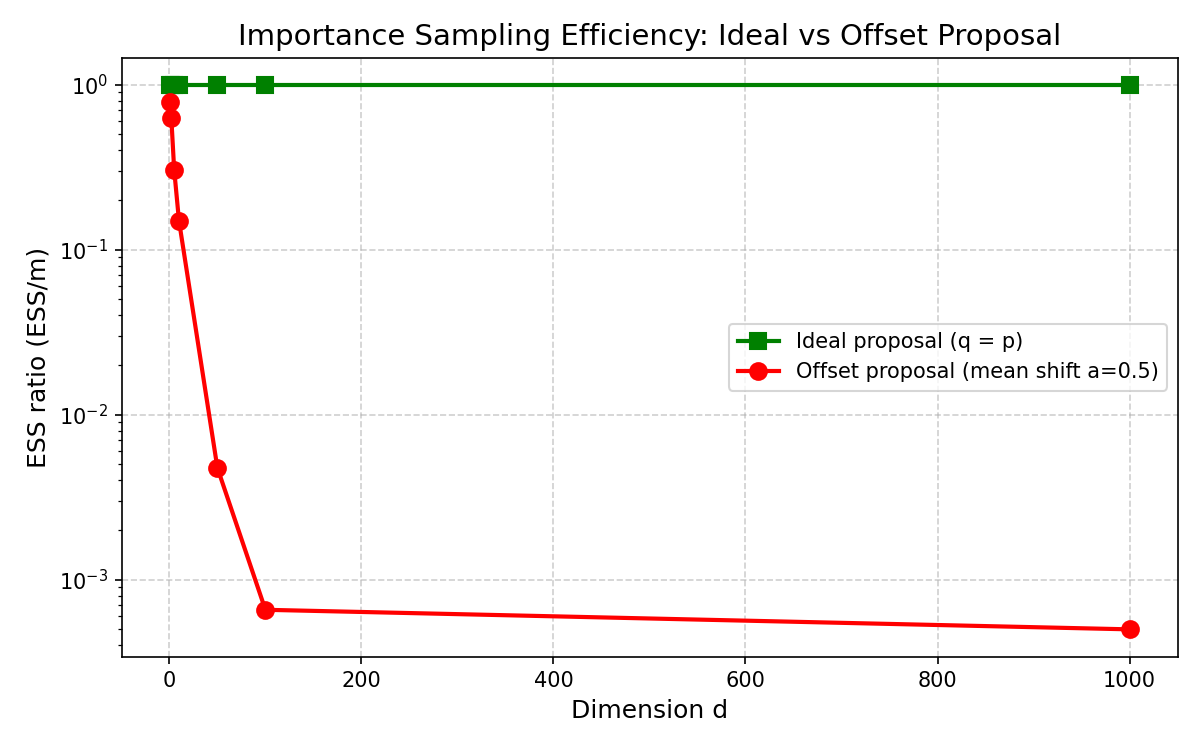
\includegraphics[width=\columnwidth]{importance_sampling_ideal_vs_offset.png}
\caption{Experiment~D: \(\mathrm{ESS}/m\) vs.\ dimension for ideal \(q=p\) vs.\ mean-shifted Gaussian (\(a=0.5\)), \(m=2000\) samples.}
\label{fig:expD}
\end{figure}

\section{DISCUSSION}
\begin{itemize}[noitemsep]
    \item Proposal design must respect the support of \(p\) and the shape of \(|f|\,p\); heavy tails often stabilize weights for tail functionals.
    \item A proposal matched to \(|f|p\) can dramatically reduce variance (Experiment~A); a poor proposal can perform worse than direct sampling under \(p\).
    \item Self-normalized IS avoids needing \(Z\) but introduces bias at finite \(N\); our mixture experiment shows it remains practical when \(q\) has adequate coverage.
    \item High-dimensional mismatch between \(p\) and \(q\) drives ESS toward zero (Experiment~D); mitigations include tempered proposals, annealed IS, transport maps, and sequential Monte Carlo.
    \item Advanced directions include adaptive proposals, multiple IS, and particle filters.
\end{itemize}

\section{CONCLUSION}
Importance Sampling is a flexible Monte Carlo tool: the same estimator either gains enormous efficiency or fails visibly depending on \(q\). Our experiments tie this to variance, weight histograms, acceptance in rejection sampling, and ESS in dimension. Despite limitations in high dimensions, IS remains central to off-policy evaluation, Bayesian computation, and rare events in AI.

\section{REFERENCES}
\begin{enumerate}[label={[\arabic*]}]
    \item C. P. Robert and G. Casella, \emph{Monte Carlo Statistical Methods}. Springer, 2004.
    \item M. Sugiyama, \emph{Statistical Reinforcement Learning}. Chapman \& Hall/CRC, 2016.
    \item A. B. Owen, \emph{Monte Carlo Theory, Methods and Examples}. 2013.
\end{enumerate}

\end{document}
